% ===============================================================================
% = LaTeX Beamer Template des Arbeitsbereichs Sicherheit in verteilten Systemem
% = (c) 2012 Prof. Dr. Hannes Federrath, Uni Hamburg, Fachbereich Informatik
% = http://www.informatik.uni-hamburg.de/svs/
% ===============================================================================
%
\documentclass[t]{beamer} 
% Option t              Place text of slides at the (vertical) top of the slides.
% Option handout        Ein PDF ohne Pausen und Overlayeffekte erzeugen.
% Option aspectratio=43 169 => 16:9, 1610 => 16:10, 43 => 4:3
\usepackage[utf8]{inputenc}
\usepackage[ngerman]{babel}
\usepackage{graphicx,xcolor}
\usepackage[T1]{fontenc} % 8-Bit-Zeichen; ermöglicht korrektes Kopieren von Umlauten aus dem pdf 
\usepackage[scaled]{helvet}

\usepackage{tikz}
\usetikzlibrary{positioning}

\usepackage[normalem]{ulem}

\usepackage{beamerthemedefault}

% Ränder definieren
\setbeamersize{text margin left=5ex, text margin right=5ex}

% Farbdefinitionen
\definecolor{svsgrau1}{RGB}{191,191,191} % Balken in Kopfzeile
\definecolor{svsgrau2}{RGB}{123,123,123} % Folienüberschriften
\definecolor{svsrot}{RGB}{255,0,0} % Bullets
\definecolor{svshellblau1}{RGB}{153,204,255} % Block Hintergrund
\definecolor{svshellblau2}{RGB}{24,113,248} % Anstrich Ebene 2
\definecolor{svsdunkelblau}{RGB}{38,82,128} % Text der Ebene 1

% Navigationsleiste ausblenden
\beamertemplatenavigationsymbolsempty 

% Farben der Bullets der Ebenen
\setbeamercolor{itemize item}{fg=svsrot}
\setbeamercolor{itemize subitem}{fg=svshellblau2}
\setbeamercolor{enumerate item}{parent=itemize item}
\setbeamercolor{enumerate subitem}{parent=itemize subitem}

% Formen der Bullets der Ebenen
\setbeamertemplate{itemize item}[circle] 
\setbeamertemplate{itemize subitem}{--} 
\setbeamertemplate{itemize subsubitem}[circle] 

% Farben der Texte 
\setbeamercolor{title}{fg=black}
\setbeamercolor{structure}{fg=svsgrau2}
\setbeamercolor{section in toc}{fg=black}
\setbeamercolor{framesubtitle}{fg=svsdunkelblau}
\setbeamercolor{itemize/enumerate body}{fg=svsdunkelblau}
\setbeamercolor{itemize/enumerate subbody}{fg=black}
\setbeamercolor{itemize/enumerate subsubbody}{fg=black}

% Zeichensätze der Texte
\setbeamerfont{author}{size=\normalsize}
\setbeamerfont{institute}{size=\normalsize}
\setbeamerfont{date}{size=\normalsize}
\setbeamerfont{frametitle}{size=\large}
\setbeamerfont{framesubtitle}{size=\footnotesize\raggedleft}
\setbeamerfont{sections/subsections in toc}{size=\normalsize}
\setbeamerfont{itemize/enumerate body}{size=\normalsize}
\setbeamerfont{itemize/enumerate subbody}{size=\normalsize}
\setbeamerfont{itemize/enumerate subsubbody}{size=\normalsize}

% Definitionen für farbig hinterlegten Block 
\setbeamertemplate{blocks}[rounded]
\setbeamercolor{block title}{fg=black,bg=svshellblau1}
\setbeamercolor{block body}{parent=normal text,use=block title,bg=block title.bg!25!bg}
\setbeamerfont{block title}{size=\normalsize}
\setbeamerfont{block body}{size=\normalsize}

% Definitionen für Agenda (FIXME: noch stärker an normale Listendefs. anpassen)
\setbeamertemplate{section in toc}[sections numbered]
\setbeamertemplate{subsection in toc}[square]

% Kopfzeile
\setbeamertemplate{headline}{
	
\includegraphics[height=8mm]{pic/UHH-Logo_2010_ohneText.png}%
	\color{svsgrau1}\rule{\paperwidth}{8mm}\newline
	\mbox{}\rule{1em}{0pt}\rule{0pt}{8ex}
	\dotfill\newline\vspace{-7.3ex}
}

% Fusszeile
\setbeamertemplate{footline}[text line]{
	\parbox[b]{50mm}{\insertframenumber\\[1ex]}
}

% Hintergrund Titelseite
\defbeamertemplate{background canvas}{titlepage}{%
	{\color{svsgrau1}\vrule width\paperwidth height0.7\paperheight}%
	{\color{white}\vrule width\paperwidth height0.3\paperheight}%
}

% =============================
% = Ab hier Inhalte ändern... 
% =============================

\title{k-Anonymität}
\author[]{Thomas Maier, Kai Sonnenwald, Tom Petersen}
\institute[Uni Hamburg]{Universität Hamburg\\ Fachbereich Informatik}
\date{}

\begin{document}

\begingroup
	\setbeamertemplate{background canvas}[titlepage]
	\begin{frame}[plain]
		\vskip8mm
		
\includegraphics[width=2.2cm]{pic/svs_logo_hires-ohne-was.png}
		% \vskip-20mm % dies geht nur bei kurzen Vortragstiteln
		\titlepage
		\vspace{\fill}
		
\includegraphics[width=2.9cm]{pic/UHH-Logo_2010_Farbe_RGB_hires_nomargin.png}
		\vskip20pt
	\end{frame}
\endgroup

\begin{frame}{Agenda}
	\tableofcontents
\end{frame}

\section{Motivation \& Abgrenzung}

\begin{frame}{Anonym?}
	\begin{figure}%[ht]
		\centering
		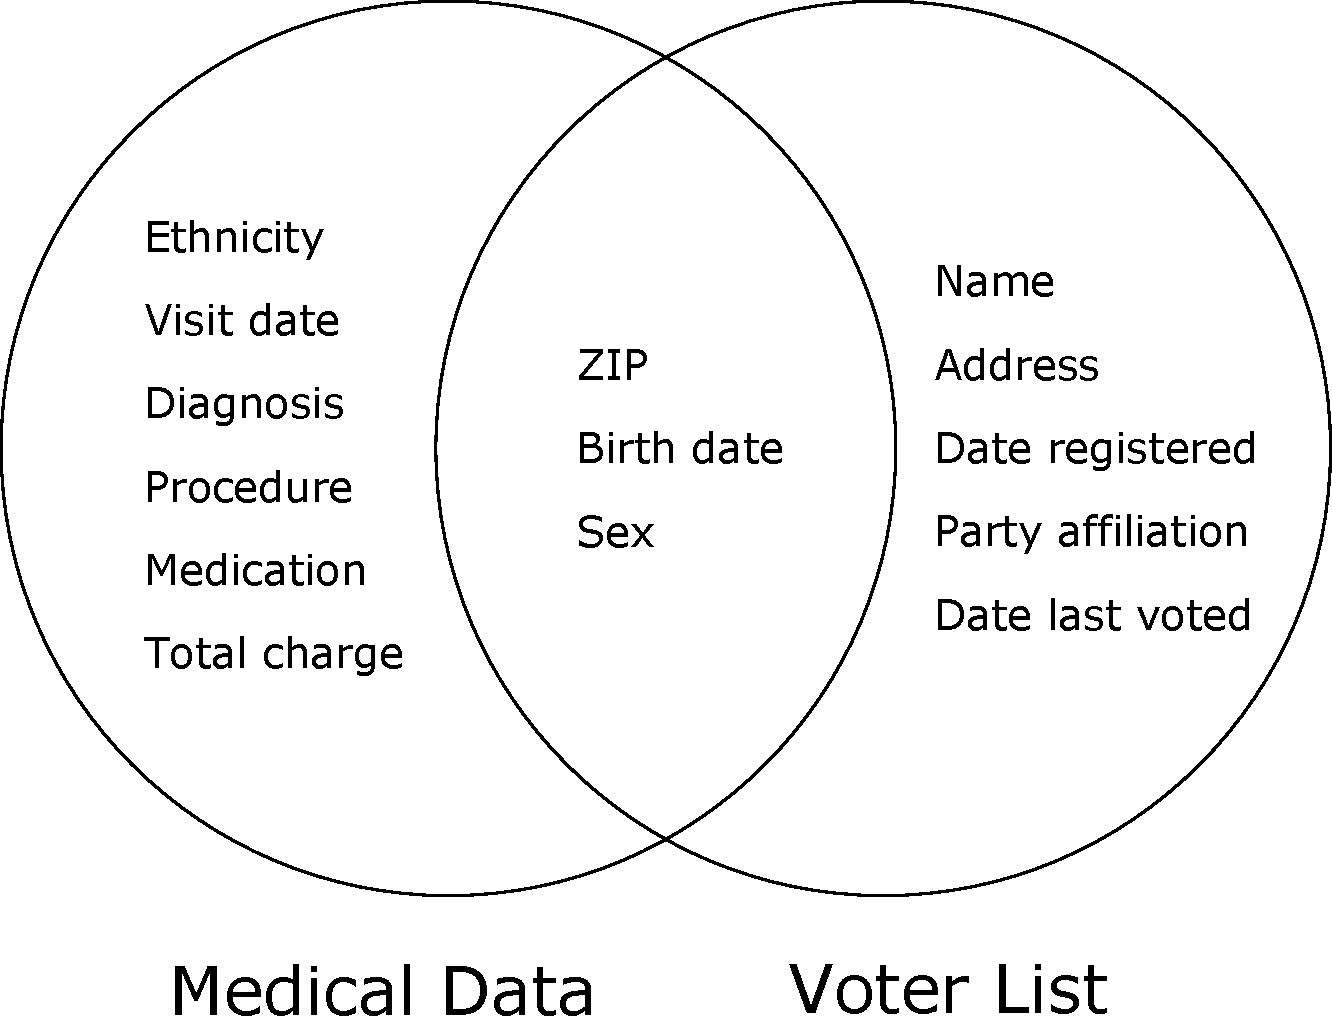
\includegraphics[width=0.7\textwidth]{pic/sweeney_governor.pdf}
		\vspace{0.2cm}
	
		\tiny Massachusetts Group Insurance Commission (GIC) medical data and voter registration data. Entnommen aus \cite{sweeney_k_anonymity}.
	\end{figure}

	%Sweeney - Beispiel \cite{sweeney_k_anonymity}
	%
	%---
	%
	%- Group Insurance Commission veröffentlichte Patientendaten in anonymer Form
	%
	%- Cambridge, Massachusetts voter registration list mit den öffentlichen Informationen der GIC abgeglichen
	%
	%- Beispielsweise konnte Massachusetts governor William Weld eindeutig identifiziert werden.
\end{frame}

\begin{frame}{Anonym? II}
	Sweeney \cite{sweeney_demographics}(1990) und Golle \cite{golle_demographics}(2000) überprüften die Eindeutigkeit von demographischen Faktoren in der Bevölkerung der USA.
	
	%	Sweeney für die 1990 US census data, Golle wiederholte das für 2000
	%
	%\begin{center}
	%	\begin{tabular}{|r|r|r|r|r|}
	%	\hline	 & \textbf{Geb.dat.} & \textbf{M. \& J.} & \textbf{J.} & \textbf{2 J.} \\
	%	\hline \textbf{PLZ} & 87.1 & 3.7 & 0.04 & 0.01 \\
	%	\hline \textbf{Ort} & 58.4 & 3.6 & 0.04 & 0.01 \\
	%	\hline \textbf{County} & 18.1 & 0.04 & 0.00004 & 0.00000 \\
	%	\hline
	%	\end{tabular}
	%\end{center}
	
	\begin{center}
		\begin{tabular}{|r|r|r|r|r|}
		\hline	 & \textbf{T. M. J.} & \textbf{M. J.} & \textbf{J.} & \textbf{2 J.} \\
		\hline \textbf{PLZ} & 87.1 \% & 3.7 \% & 0.04 \% & 0.01 \% \\
		\hline \textbf{Ort} & 58.4 \% & 3.6 \% & 0.04 \% & 0.01 \% \\
		\hline \textbf{County} & 18.1 \% & 0.04 \% & 0.00004 \% & 0.00000 \% \\
		\hline
		\end{tabular}
		\vspace{0.2cm}
	
		\tiny Eindeutig identifizierbarer Individuenanteil an der U.S.-Bevölkerung 1990. Entnommen aus \cite{sweeney_demographics}.
	\end{center}

	\textbf{Ergebnis}: Durch \{Geburtsdatum, Geschlecht, PLZ\} könnten ~87\% der Bevölkerung eindeutig identifiziert werden.
		
	%	
	%	---
	%	
	%	Basierend auf den Daten, die folgende Felder darstellen (aggregiert): 
	%	
	%	StateID 	State Code 
	%	ZIP 		5-digit ZIP 
	%	TotPop 		Total Population 
	%	AUnder12 	Population Under Age 12 Years 
	%	A12to18 	Population Age 12-18 Years 
	%	A19to24 	Population Age 19-24 Years 
	%	A25to34 	Population Age 25-34 Years 
	%	A35to44 	Population Age 35-44 Years 
	%	A45to54 	Population Age 45-54 Years 
	%	A55to64 	Population Age 55-64 Years 
	%	A65Plus 	Population Age 65 Years and up 
	%	
	%	Betrachtet wird jeweils die Anzahl unterschiedlicher möglicher unterschiedlicher Werte, die sich für die entsprechenden Attribute ergeben und die tatsächliche Anzahl der Population. Wenn die Anzahl möglicher Ausprägungen die tatsächliche Population übertrifft, dann werden die Individuen als eindeutig identifizierbar angesehen, ansonsten nicht -> Grobe Abschätzung.
\end{frame}

\begin{frame}{Abgrenzung}

Vermeintlich anonyme Daten stellen sich als nicht anonym heraus. \textbf{Daher}: wie können wir Aussagen über die "'Güte"' der Anonymisierung machen?

\vspace{0.5cm}
\pause

Worum es nicht gehen soll:

\begin{itemize}
	\item Begrenzung des Zugriffs (Authentifikation, Multi-Level-Datenbanken)
	\item Statistische Datenbanken (Aggregation, Begrenzung von Selektionsarten, Logging und Abwägen von Anfragen, Hinzufügen von Zufall)
\end{itemize}

Darum geht es:

\begin{itemize}
	\item Veröffentlichung von Daten als Individualdatensätze ohne Integritätsverlust unter Wahrung der Anonymität.
\end{itemize}

\end{frame}


\section{k-Anonymität}

\begin{frame}{k-Anonymität}
Notizen

identifier, quasi-identifier, sensitive attributes

k-anonymity
\end{frame}

\begin{frame}{Begriffe}
	\begin{description}
	\item[Explicit identifier] Attribut, das ein Individuum (nahezu) eindeutig identifiziert. Bsp: Name, Adresse, Steuernummer, ...
	\item[Quasi identifier] Attributmenge, die ein Individuum in Kombination identifizieren kann. \textit{Formal in \cite{sweeney_k_anonymity} p. 7}, auch \cite{machanavajjhala_l_diversity} p. 3
	\item[Sensitive attribute] Attribut, dessen Wert für ein Individuum in einer Datenmenge nicht herausgefunden werden darf.
	\end{description}
\end{frame}

\begin{frame}{k-Anonymität}
	\textbf{Informell}: Eine Tabelle (Datensatz?) erfüllt \(k\)-Anonymität, wenn jede Zeile (jeder Eintrag) ununterscheidbar von \(k-1\) anderen Zeilen im Bezug auf jeden "'quasi identifier"'-Menge ist.

	\vspace{0.5cm}

	\textbf{Formal}: Sei \(T(A_1, \dots , A_n)\) eine Tabelle und \(Q_T=\{A_i, \dots, A_j\}\) der zugehörige quasi identifier. \(T\) erfüllt \(k\)-Anonymität genau dann, wenn jede Belegung von Werten in \(T[Q_T]\) mindestens \(k\) mal auftritt, wobei \(T[Q_T]\) die duplikatenerhaltende Projektion von \(T\) auf die Attribute des quasi identifiers beschreibt.
\end{frame}

\subsection{Generalisierung}

\begin{frame}{Generalisierung}
	\textbf{s. Samarati, Sweeney Kapitel 3}
	
	domain, ground domain, generalization (partial ordering on domains)
	
	generalized table
\end{frame}

\subsection{Unterdrückung}

\begin{frame}{Suppression}
	...
	
	in combination with generalization
\end{frame}

\section{Schwächen der k-Anonymität}

\begin{frame}{Schwächen der k-Anonymität}

\begin{description}
	\item[Unsorted matching attack] Veröffentlichung mehrerer \(k-\)anonymer Tabellen mit derselben Sortierung ausgehend von einer nicht-öffentlichen Tabelle. \cite{sweeney_k_anonymity} p.10
	\item[Complementary release attack] Veröffentlichung mehrerer \(k-\)anonymer Tabellen unterschiedlicher Generalisierung, die zusammengeführt die \(k-\)Anonymität verletzen. \cite{sweeney_k_anonymity} p.11
	\item[Temporal attack] Dynamische Tabellen können \(k-\)Anonymität verletzen. \cite{sweeney_k_anonymity} p.12
	\item[Homogeneity attack] Gleichheit der sensitive attributes einer Gruppe, die sich in den Werten des quasi identifiers gleicht, leakt das sensitive attribute eines Individuums. \cite{machanavajjhala_l_diversity} p. 2
	\item[Background knowledge attack] Nutzen von Hintergrundwissen, um mit hoher Wahrscheinlichkeit auf den Wert des sensitive attributes eines Individuumsin einer Gruppe zu schließen. \cite{machanavajjhala_l_diversity} p.2/4
\end{description}

\end{frame}

\section{l-Diversity}

\begin{frame}{l-Diversity - Prinzip}

\begin{description}
	\item[Prinzip] Eine Tabelle erfüllt \(l\)-Diversity, wenn in jedem \(k\)-anonymen Block mindestens \(l\) verschiedene Werte für das sensitive Attribut vorkommen.
    
    \vspace{1.0cm}
    
    \item[Bsp.-Tabelle]
    \small
	\begin{tabular}{|c|c|c|}
	\hline \textbf{G.jahr} & \textbf{PLZ} & \textbf{Erkrankung} \\
	\hline
     1970 & 21*** & Hepatitis X \\ 
	 1970 & 21*** & Hepatitis Y \\ 
	 1970 & 21*** & Hepatitis Z \\
	\hline 
     1975 & 21*** & Hepatitis X \\
     1975 & 21*** & Hepatitis X \\ 
	 1975 & 21*** & Hepatitis X \\ 
	\hline 
	\end{tabular}
	\vspace{0.3cm}

	\(k = 4, l = 1\)
\end{description}

\end{frame}


\begin{frame}{l-Diversity - Definitionen}
	\begin{block}{l-Diversity - Entropie basiert}
    \centering
        Eine Tabelle ist \(l\)-divers, wenn für jeden $q*$-Block die folgende Ungleichung erfüllt wird:
        
    	$\sum\limits_{s \in S} p_{(q^*,s)} log(p_{(q^*,s')}) \geq log(l)$
        
    	Dabei stellt $p_{(q^*,s)}$ den Anteil des Werts $s$ in dem $q^*$-Block dar.
   \end{block}
    \tiny Definition nach \cite{machanavajjhala_l_diversity}.
    
    \vfill
    
	\begin{block}{l-Diversity - rekursiv}
    \centering
		Innerhalb eines $q^*$-Blocks sei $r_i$ die Anzahl des $i$-häufigsten sensiblen Attributs. Mit einer gegebenen Konstante $c$ erfüllt dieser $q^*$-Block rekursive $(c, l)$-Diversity, wenn $r_1 < c(r_l + r_{l+1} + ...  + r_m )$ gilt. Eine Tabelle $T^*$ erfüllt $(c, l)$-Diversity, wenn jeder $q^*$-Block $(c, l)$-Diversity erfüllt. $1$-Diversity ist immer erfüllt.
    \end{block}
    \tiny Definition nach \cite{machanavajjhala_l_diversity}.
\end{frame}


\begin{frame}{Beispiel: 2-diverse Tabelle}
	\begin{center}
		%Erstellt von script/generate_table.py - bei Bedarf anpassen
			\begin{tabular}{|l|c|c|r|l|}
		\hline \textit{Identifier} & \multicolumn{3}{c|}{\textbf{Nicht-sensibel}} & \textbf{Sensibel} \\ 
		\hline \textit{Name} & \textbf{Geschl.} & \textbf{PLZ} & \textbf{Geburtsjahr} & \textbf{Erkrankung} \\ \hline
		\hline \rowcolor{svshellblau1!30} 	- & w & 22*** & 1944-45 & Hepatitis \\ 
		\hline \rowcolor{svshellblau1!30}	- & w & 22*** & 1944-45 & Gicht \\ 
		\hline \rowcolor{svsgrau1!30} 		- & * & 22*** & 1949 & Arthrose \\ 
		\hline \rowcolor{svshellblau2!30} 	- & w & 228** & 1985-92 & Diabetes \\
		\hline \rowcolor{svshellblau2!30} 	- & w & 228** & 1985-92 & Demenz \\  
		\hline \rowcolor{white} 		- & m & 22997 & 1936-75 & Arthrose \\ 
		\hline \rowcolor{svsgrau1!30} 		- & * & 22*** & 1949 & Diabetes \\ 
		\hline \rowcolor{svsrot!30} 		- & m & 22*** & 1963-64 & Demenz \\ 
		\hline \rowcolor{svsrot!30} 		- & m & 22*** & 1963-64 & Demenz \\ 
		\hline \rowcolor{white} 		- & m & 22997 & 1936-75 & Hepatitis \\ 
		\hline 
		\end{tabular}
		\vspace{0.5cm}
        
		k-anonyme Tabelle mit \(k=2\), aber nur l-divers mit \(l=1\)
	\end{center}
\end{frame}


\begin{frame}{Beispiel: 2-diverse Tabelle}
	\begin{center}
		%Erstellt von script/generate_table.py - bei Bedarf anpassen
			\begin{tabular}{|l|c|c|r|l|}
		\hline \textit{Identifier} & \multicolumn{3}{c|}{\textbf{Nicht-sensibel}} & \textbf{Sensibel} \\ 
		\hline \textit{Name} & \textbf{Geschl.} & \textbf{PLZ} & \textbf{Geburtsjahr} & \textbf{Erkrankung} \\ \hline
		\hline \rowcolor{svshellblau1!30} 	- & w & 22*** & 1944-45 & Hepatitis \\ 
		\hline \rowcolor{svshellblau1!30}	- & w & 22*** & 1944-45 & Gicht \\ 
		\hline \rowcolor{svsgrau1!30} 		- & * & 22*** & 1949 & Arthrose \\ 
		\hline \rowcolor{svshellblau2!30} 	- & w & 228** & 1985-92 & Diabetes \\
		\hline \rowcolor{svshellblau2!30} 	- & w & 228** & 1985-92 & Demenz \\  
		\hline \rowcolor{svsrot!30} 		- & m & 22*** & 1936-75 & Arthrose \\ 
		\hline \rowcolor{svsgrau1!30} 		- & * & 22*** & 1949 & Diabetes \\ 
		\hline \rowcolor{svsrot!30} 		- & m & 22*** & 1936-75 & Demenz \\ 
		\hline \rowcolor{svsrot!30} 		- & m & 22*** & 1936-75 & Demenz \\ 
		\hline \rowcolor{svsrot!30} 		- & m & 22*** & 1936-75 & Hepatitis \\ 
		\hline 
		\end{tabular}
		\vspace{0.5cm}
        
		\textbf{Ergebnis:} k-anonyme Tabelle mit \(k=2\) und l-divers mit \(l=2\)
	\end{center}
\end{frame}


\subsection{Verbesserung zu k-Anonymität}

\begin{frame}{Verbesserung zu k-Anonymität}
- $l$-Diversität verteilt die gleichen sensiblen Attribute auf die verschiedenen Blöcke.\\
\ \\ => Somit ist eine \textit{Homogenity Attack} nicht mehr möglich.\\
\ \\ => Eine \textit{Background Knowledge Attack} wird erschwert.\\
\ \\ \tiny \cite{machanavajjhala_l_diversity}

\vspace{1.0cm}

\normalsize
- Ein Vorteil von l-Diversity ist, dass vorhandene Generalisierungsalgorithmen leicht angepasst werden können.

\end{frame}


\subsection{l-Diversität Schwächen}

\begin{frame}{l-Diversität - Schwächen}

\begin{description}
	\item[Skewness Attack] \ \\
    - Tabelle mit 1 sensiblen Attribut, 2 Ausprägungen.\\
    - Wahrscheinlichkeit für Wert 1 ist sehr hoch.\\
    - Wahrscheinlichkeit für Wert 2 entsprechend niedrig.\\
    - 2-diverse Tabelle mit Block $q^*$\\
    - $q^*$ Beinhaltet zu 50\% Wert 1 und zu 50\%  Wert 2\\
    - Die Wahrscheinlichkeit, dass ein Tupel aus q* den Wert 2 hat liegt nun bei 50\%  \\
    \tiny \cite{Li2007t-closseness}. 
\end{description}
\vspace{0.5cm}

\textbf{Beispiel:} Angenommen das sensible Attribut hat die Werte: krank / gesund. In der Bevölkerung sind 1\% krank und 99\% gesund. Die Wahrscheinlichkeit, dass eine Person aus dem Block $q^*$ krank ist liegt nun bei 50\% und nicht mehr bei 1\%.
\end{frame}

\begin{frame}{l-Diversität - Schwächen}
\begin{description}	
	\item[Similarity Attack] l-Diversity garantiert, dass in jedem Block unterschiedliche sensible Werte stehen. Es kann jedoch vorkommen, dass sich diese Werte ähneln. \\
    \tiny \cite{Li2007t-closseness} 
\end{description}

\vspace{1.5cm}

\normalsize
\textbf{Beispiel:} In einem Block stehen unterschiedliche Krankheiten als sensitives Attribut. Es sind nur Geschlechtskrankheiten.

Wenn nun eine Person diesem Block zugeordnet werden kann, so weiß man auch, dass diese Person eine Geschlechtskrankheit hat.

\end{frame}


\section{t-Closeness}

\begin{frame}{t-Closeness}
	t-closeness stellt ein Maß für minimalen Wissensgewinn, der durch Betrachtung eines q*-Blocks im Vergleich zur gesamten Distribution entsteht, dar \cite{kltHauf}.

	\begin{block}{Definition t-closeness}
		Eine \textbf{Äquivalenzklasse} (q*-Block) hat die Eigenschaft \textbf{t-closeness}, wenn die (semantische) Distanz zwischen der Verteilung der Werte eines sensiblen Attributes innerhalb der Äquivalenzklasse und der Verteilung der Werte des sensiblen Attributes innerhalb der Tabelle nicht größer als \(t\) ist. 

		Eine \textbf{Tabelle} hat die Eigenschaft \textbf{t-closeness}, wenn diese Eigenschaft für alle Äquivalenzklassen erfüllt ist.	
	\end{block}

	\textbf{Problem}: Wie bestimmt man die (semantische) Distanz?
\end{frame}

\subsection{Earth Movers Distanz (EMD)}

\begin{frame}{Earth Movers Distanz (EMD)}
	Die Earth Movers Distanz (EMD) basiert auf der minimalen Arbeit, die zu verrichten ist, um eine Verteilung in eine andere umzuwandeln.
	\begin{block}{Definition von EMD \cite{Li2007t-closseness}}
		Gegeben sei $P=(p_1,...,p_m)$, $Q=(q_1,...,q_m)$, $d_{ij}$ ist die Grunddistanz zwischen $p_i$ und $q_j$. $f_{ij}$ ist die minimale Masse, die transportiert werden muss um $p_i$ in $q_i$ zu verwandeln. EMD ist dann die gesamte Arbeit die verrichtet werden muss $D[P,Q] = \sum_{i=1}^m \sum_{j=1}^m d_{ij} f_{ij}$.\\
		Unter den folgenden Bedingungen
		\begin{enumerate}[i)]
			\item $f_{ij}\ge 0$ | $1\le i \le m, 1\le j \le m$		
			\item $p_i - \sum_{j=1}^{m}f_{ij} +\sum_{j=1}^{m}f_{ji} = q_i$ | $1 \le i \le m$
			\item $\sum_{i=1}^{m}\sum_{j=1}^{m} f_{ij} = \sum_{i=1}^{m} p_i = \sum_{i=1}^{m} q_i$ 
		\end{enumerate}
	\end{block}
\end{frame}

\begin{frame}{Earth Movers Distanz (EMD)}
	Aus den drei Bedingungen folgen die zwei Fakten \cite{Li2007t-closseness}:\\
	\ \\
	\textbf{Fakt 1:} If $\forall i,j | 0 \le d_{ij} < 1$ then $0 \le D[P,Q]  \le 1$. 
	Das Bedeutet, dass wenn die Grunddistanz normalisiert ist, ist auch der EMD normalisiert. \textbf{Somit kann ein einheitliches Maß für t bestimmt werden.}\\
	\ \\
	\textbf{Fakt 2:} Gegeben sind zwei Äquivalenzklassen $E_1$ und $E_2$.
	$P_1$ ist die Verteilung eines sensitiven Attributes aus $E_1$.
	$P_2$ ist die Verteilung eines sensitiven Attributes aus $E_2$.
	$P$ ist die Verteilung eines sensitiven Attributes aus $E_1 \cup E_2$. Dann gilt die folgende Ungleichung: \\
	$D[P,Q] \le \frac{|E_1|}{|E_1|+|E_2|}D[P_1,Q] + \frac{|E_2|}{|E_1|+|E_2|}D[P_2,Q]$\\
	$\Rightarrow D[P,Q] \le max(D[P_1,Q], D[P_2,Q])$ 
\end{frame}

\begin{frame}{Earth Movers Distanz (EMD)}
	\textbf{Fakt 2:} $D[P,Q] \le max(D[P_1,Q], D[P_2,Q])$ 
	Dies Bedeutet, dass die maximale Distanz zwischen einer Äquivalenzklasse und der Tabelle beim zusammenführen zweier Äquivalenzklassen nicht steigt. \textbf{Somit bleibt die t-closeness Eigenschaft beim zusammenführen erhalten.} \\ 
	\ \\
	\textbf{Generalisation Property:} Sei $T$ eine Tabelle, $A$ und $B$ sind Generalisierungen von $T$, wobei$A$ mehr generalisiert ist als $B$. Wenn $B$ die Eigenschaft t-closeness hat, dann hat auch $A$ die Eigenschaft t-closeness.\\
	\ \\
	\textit{Beweis:} Die Äquivalenzklassen aus $A$ bestehen aus der vereinigung mehrerer Äquivalenzklassen aus $B$. Nach Fakt 2 kann somit maximale Distanz nicht größer werden. Somit hat auch $A$ die Eigenschaft t-closeness.  
\end{frame}

\begin{frame} {EMD Beispiel}
	
	\begin{columns}[T]
		\begin{column}{0.5\textwidth}
			\begin{table}[]
				\centering
				\label{tclossenessExample}
				\begin{tabular}{|l|l|l|}
					\hline
					\textbf{PLZ}   & \textbf{Alter}    & \textbf{Einkommen} \\\hline
					4767* & $\le 40$ & 3K \\
					4767* & $\le 40$ & 4K \\
					4767* & $\le 40$ & 5K \\\hline
					4790* & $\ge 40$ & 6K \\
					4790* & $\ge 40$ & 8K \\
					4790* & $\ge 40$ & 11K \\\hline
					4760* & $\le 40$ & 7K \\
					4760* & $\le 40$ & 9K \\
					4760* & $\le 40$ & 10K \\\hline
				\end{tabular}
				\caption{Einkommenstabelle}
			\end{table}
		\end{column}
		
		\begin{column}{0.5\textwidth}
			$Q = \{3k, 4k, 5k, 6k, 7k, 8k, 9k, 10k, 11k\}$\\
			\ \\
			$P_1 = \{3k, 4k, 5k\}$ \\
			$P2 = (\{6k, 8k, 11k\})$ 
			$P3 = (\{7k, 9k, 10k\})$
			\ \\
			\ \\
			\tiny Beispiel aus \cite{Li2007t-closseness}
		\end{column}
	\end{columns}
\end{frame}
\subsection{EMD Formeln} 
\begin{frame}{EMD Formeln}
	\textbf{Nummerische Attribute:} \\
	Domäne: $\{v_i,...,v_m\}$, wobei gilt $i<j \Rightarrow v_i \le v_j$\\
	\ \\
	geordnete-Distanz($v_i,v_j$)= = $\frac{|i-j|}{m-1}$
\end{frame}
\begin{frame}{EMD Formeln}
	\begin{figure}
		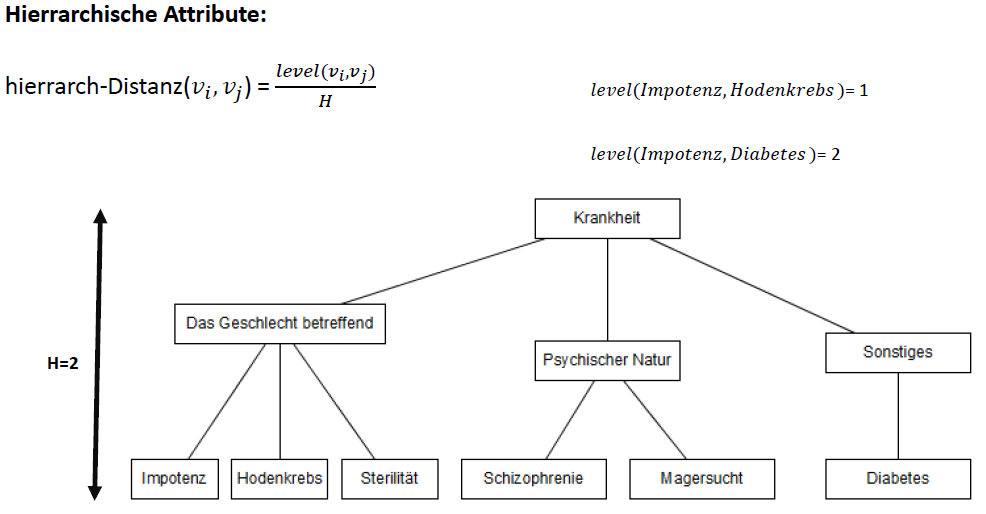
\includegraphics[scale=0.45]{pic/EMD_Formel.png}
	\end{figure}
\end{frame}
\subsection{EMD Beispiel}
\begin{frame}{EMD Beispiel}
	$Q = \{3k, 4k, 5k, 6k, 7k, 8k, 9k, 10k, 11k\}$\\
	$P_1 = \{3k, 4k, 5k\}$ \\
	Wahrscheinlichkeit $\frac{1}{9}$ für folgende Transition:
	$(5k\rightarrow 11k), (5k\rightarrow 10k), (5k \rightarrow 9k),
	(4k \rightarrow 8k), (4k\rightarrow 7k), (4k \rightarrow 6k), (3k\rightarrow 5k), (3k\rightarrow 4k), (3k \rightarrow 3k).$\\
	\ \\
	$\Rightarrow D[P_1,Q]= \frac{1}{9} \cdot \frac{6 + 5 + 4 + 4 + 3 + 2 + 2 + 1 + 0}{9-1} = 27/72 = 3/8 = 0.375$
\end{frame}
\begin{frame} {EMD Beispiel}
	
	\begin{columns}[T]
		\begin{column}{0.5\textwidth}
			\begin{table}[]
				\centering
				\label{tclossenessExample}
				\begin{tabular}{|l|l|l|}
					\hline
					\textbf{PLZ}   & \textbf{Alter}    & \textbf{Einkommen} \\\hline
					4767* & $\le 40$ & 3K \\
					4767* & $\le 40$ & 4K \\
					4767* & $\le 40$ & 5K \\\hline
					4790* & $\ge 40$ & 6K \\
					4790* & $\ge 40$ & 8K \\
					4790* & $\ge 40$ & 11K \\\hline
					4760* & $\le 40$ & 7K \\
					4760* & $\le 40$ & 9K \\
					4760* & $\le 40$ & 10K \\\hline
				\end{tabular}
				\caption{Einkommenstabelle}
			\end{table}
		\end{column}
		
		\begin{column}{0.5\textwidth}
			$D[P_1,Q]=\frac{27}{72} = 0,375$\\
			\ \\
			$D[P_2,Q]=\frac{12}{72} = 0,167$\\
			\ \\
			$D[P_3,Q]=\frac{17}{72} = 0,236,$\\
			\ \\
			$\Rightarrow t=0,375$\\
			\ \\
			Die Einkommenstabelle hat die Eigenschaft 0,375-closeness	
		\end{column}
	\end{columns}
\end{frame}
\begin{frame} {EMD Beispiel}
	
	\begin{columns}[T]
		\begin{column}{0.5\textwidth}
			\begin{table}[]
				\centering
				\label{tclossenessExample}
				\begin{tabular}{|l|l|l|}
					\hline
					\textbf{PLZ}   & \textbf{Alter}    & \textbf{Einkommen} \\\hline
					4767* & $\le 40$ & 3K \\
					4767* & $\le 40$ & 5K \\
					4767* & $\le 40$ & 9K \\\hline
					4790* & $\ge 40$ & 6K \\
					4790* & $\ge 40$ & 8K \\
					4790* & $\ge 40$ & 11K \\\hline
					4760* & $\le 40$ & 4K \\
					4760* & $\le 40$ & 7K \\
					4760* & $\le 40$ & 10K \\\hline
				\end{tabular}
				\caption{Einkommenstabelle}
			\end{table}
		\end{column}
		
		\begin{column}{0.5\textwidth}
			$D[P_1^{'},Q]=\frac{12}{72} = 0,167$\\
			\ \\
			$D[P_2,Q]=\frac{12}{72} = 0,167$\\
			\ \\
			$D[P_3^{'},Q]=\frac{6}{72} = 0,083,$\\
			\ \\
			$\Rightarrow t=0,375$\\
			\ \\
			Die Einkommenstabelle hat die Eigenschaft 0,167-closeness	
		\end{column}
	\end{columns}

\end{frame}

\section{Fazit}

\begin{frame}{Fazit}
	\begin{itemize}
		\item k-Anonymität
		\begin{itemize}
			\item mindestens $k$ Tupel mit identischem Quasi-Identifikator
		\end{itemize}

		\item l-Diversität
		\begin{itemize}
			\item mindestens $l$ verschiedene sensible Werte in jeder Äquivalenzklasse
		\end{itemize}

		\item t-Closeness
		\begin{itemize}
			\item Distanz zwischen Verteilung der sensiblen Attribute einer Äquivalenzklasse und der Gesamtverteilung unterscheidet sich maximal um einen Schwellwert \(t\)
		\end{itemize}

		\pause

		\item Ausblick
		\begin{itemize}
			\item gewichtete Attribute
			\item Schwellwerte für maximale Anzahl an unterdrückten Tupeln
			\item mehrere sensible Attribute
			\item ...
		\end{itemize}
	\end{itemize}
	%	Zusätzlich (und hier nicht abgedeckt): gewichtete Attribute, Schwellwerte für maximale Anzahl an unterdrückten Tupeln, mehrere sensible Attribute, ...
\end{frame}

\section{Literaturverzeichnis}

\begin{frame}[allowframebreaks]{Literaturverzeichnis}
\nocite{*}
\bibliographystyle{alpha}
\bibliography{literature}
\end{frame}

\end{document}

\stop











%%% INHALT SVS VORLAGE %%%

\begin{frame}
	\frametitle{Der Arbeitsbereich Sicherheit in Verteilten Systemen (SVS)}
	\begin{block}{Lorem ipsum dolor}
		Lorem ipsum dolor sit amet, consectetur adipisicing elit, sed do eiusmod tempor incididunt ut labore et dolore magna aliqua. Ut enim ad minim veniam, quis nostrud exercitation ullamco laboris nisi ut aliquip ex ea commodo consequat. 
	\end{block}
	\begin{itemize}
		\item Themen
			\begin{enumerate}
				\item Privacy Enhancing Technologies (PET)
				\item Security Management \& Risk Management
				\item Security of Mobile Systems
			\end{enumerate}
		\item Weitere Informationen
			\begin{itemize}
				\item http://www.informatik.uni-hamburg.de/svs
			\end{itemize}
	\end{itemize}
\end{frame}

\begin{frame}
	\frametitle{Beispiel für eine Abbildung}
	\begin{itemize}
		\item Zweck
			\begin{itemize}
				\item Nur mit \alert{berechtigten Partnern} weiter kommunizieren
				\item Verhindert unbefugte Inanspruchnahme von Betriebsmitteln
			\end{itemize}
	\end{itemize}
	\vspace{\fill}
	\pause % Das Nachfolgende erst nach Klick einblenden...
	\begin{center}
		%\includegraphics[width=0.8\textwidth]{pic/abbildung1.pdf}
	\end{center}
\end{frame}

\begin{frame}
	\transwipe % funktioniert nur bei Anzeige mit Acrobat Reader
	\frametitle{Beispiel für eine Abbildung}
	\begin{itemize}
		\item Zweck
			\begin{itemize}
				\item Einem Kunden \emph{\color[RGB]{0,128,0} K} einen Inhalt \emph{\color{red} I} in einer bestimmten Weise zugänglich machen, ihn aber daran hindern, \emph{alles} damit tun zu können.
			\end{itemize}
	\end{itemize}
	\vspace{\fill}
	\begin{center}
	%	\includegraphics[width=0.8\textwidth]{pic/abbildung2.pdf}
	\end{center}
\end{frame}

\begin{frame}
	\frametitle{Weiteres Beispiel für eine Abbildung}
	\framesubtitle{[John Doe, 1966] }
	\begin{itemize}
		\item Voraussetzung: {\color{black} Angreifer} 
			\begin{itemize}
				\item betreibt täuschend echte Webseite der Bank
				\item bewegt den Kunden zum Besuch dieser Seite
			\end{itemize}
	\end{itemize}
	\vspace{\fill}
	\begin{center}
	%	\includegraphics[width=\textwidth]{pic/abbildung3.pdf}
	\end{center}
\end{frame}

\begin{frame}
	\frametitle{Ebenen}
	\begin{itemize}
		\item Erste Ebene
			\begin{itemize}
				\item Zweite Ebene
				\begin{itemize}
					\item Dritte Ebene
				\end{itemize}
				\item Zweite Ebene
			\end{itemize}
		\item Erste Ebene
	\end{itemize}
	\begin{enumerate}	
		\item Erste Ebene
			\begin{enumerate}
				\item Zweite Ebene
				\begin{enumerate}
					\item Dritte Ebene
				\end{enumerate}
				\item Zweite Ebene
			\end{enumerate}
		\item Erste Ebene
	\end{enumerate}
\end{frame}


\begin{frame}{Spalten}
	\begin{columns}[T]
		\begin{column}{.6\textwidth}
			\begin{itemize}
				\item Linke Spalte
				\begin{itemize}
					\item Lorem ipsum dolor sit amet, 
					\item consectetur adipisicing elit, 
					\item sed do eiusmod tempor incididunt ut 
					\item labore et dolore magna aliqua. 
				\end{itemize}
				\item Erste Ebene
				\begin{itemize}
					\item Zweite Ebene
					\item Zweite Ebene
				\end{itemize}
				\item Erste Ebene
				\begin{itemize}
					\item Zweite Ebene
					\item Zweite Ebene
				\end{itemize}
			\end{itemize}
		\end{column}		
		\begin{column}{.4\textwidth}
			\begin{center}
				\vspace{1cm}
				
\includegraphics[width=2.2cm]{pic/svs_logo_hires-ohne-was.png} \\
				Das SVS-Logo				
			\end{center}
		\end{column}
	\end{columns}	
\end{frame}